\documentclass[a4paper]{article}

\usepackage[english]{babel}
\usepackage[utf8]{inputenc}
\usepackage{multirow}
\usepackage{rotating}
\usepackage{graphicx}	

\title{TI1705 - Part II}
\author{Gerlof Fokkema - 4257286}
\date{\today}
\setcounter{section}{4}

\newtheorem{thm}{Exercise}
\setcounter{thm}{15}

\begin{document}
  \maketitle
  \section{Part III}
  
  \subsection{State Machines}
    \begin{thm}
      Create a state machine model for the state that is implicit in \textit{doc/scenarios.md}
      requirements. The state chart should specify what happens when pausing, winning, losing, etc.
    \end{thm}
    \begin{figure}[htb]
      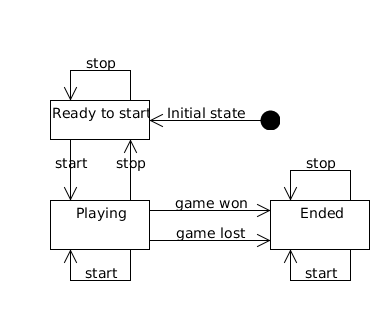
\includegraphics[height=6cm,keepaspectratio]{state}
    \end{figure}

    \begin{thm}
      Derive a transition tree from the state machine.
      Derive test cases from this transition tree, and describe them in a table.
    \end{thm}
    \begin{table}[h]
      \begin{tabular}{|l|l|l|l|}
        \hline
        Test ID & Start State & Events                                  & End State \\ \hline
        T1      & Ready       & stop                                    & Ready     \\ \hline
        T2      & Ready       & start,stop                              & Ready     \\ \hline
        T3      & Ready       & start,start                             & Playing   \\ \hline
        T4      & Ready       & start,win,stop                          & Ended     \\ \hline
        T5      & Ready       & start,win,start                         & Ended     \\ \hline
        T6      & Ready       & start,lose                              & Ended     \\ \hline
      \end{tabular}
    \end{table}
    
    \newpage
    \begin{thm}
      Compose a \textbf{state (transition)} table.
      Specify test cases for (state, event) pairs not contained in your diagram.
    \end{thm}
    \begin{table}[h]
      \begin{tabular}{|l|l|l|l|l|}
        \hline
        States  & \multicolumn{4}{|c|}{Event}        \\ \hline
                & start   & stop    & win    & lose  \\ \hline
        Ready   & Playing & Ready   &        &       \\ \hline
        Playing & Playing & Ready   & Ended  & Ended \\ \hline
        Ended   & Ended   & Ended   &        &       \\ \hline
      \end{tabular}
    \end{table}
    
    \begin{thm}
      Write a test class for the \textit{Game.game} class containing the two test suites you just derived.
      If you think you need additional test cases, explain why, and add them to your test class.
    \end{thm}
     Please refer to \textit{nl.tudelft.jpacman.game.GameTest} for the implementation of the JUnit test.
  
  \subsection{Multi-Level Games}
    \begin{thm}
      Provide an update for the scenario(s) from \textit{doc/scenarios.md} affected by the multi-level feature.
    \end{thm}
    None of the scenarios in scenarios.md are affected by the switch to multi-level games,
    since none of them test what happens when a game is stopped after it has already ended.
    Therefore we provide a new user story: \\[.2cm]
    \#\#\#\# Story 5: Start a new level \\[.4cm]
    As a player, \\
     I want to be able to start a new level \\
    After I have won a previous level \\[.4cm]
    Scenario S5.1: Start a new level. \\
    Given the player has won less than 3 times \\
    When  the player clicks the "Start" button; \\
    Then  a new level is started. \\[.4cm]
    Scenario S5.2: Player has won 3 times. \\
    Given the player has won than 3 times \\
    When  the player hits the "Start" button; \\
    Then  no new level is started \\

    \newpage
    \begin{thm}
      Adjust the statemachine from Excercise 16 so that it accommodates the multiple level functionality.
    \end{thm}
    \begin{figure}[htb]
      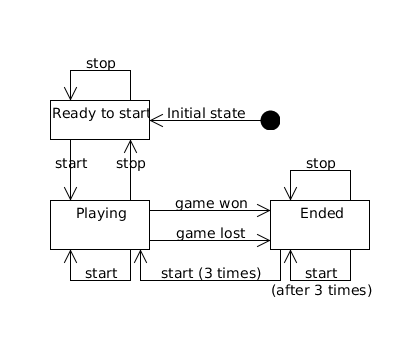
\includegraphics[height=6cm,keepaspectratio]{state-multi}
    \end{figure}

    \begin{thm}
      Derive new test cases for this new state machine.
      Which test cases that you earlier designed can be reused? Which ones must be adjusted?
    \end{thm}
    
    \begin{thm}
      Create a new top level MultiLevelLauncher (in the \textit{src} folder of your own solution),
      which is a subclass of the framework’s Launcher.
      For now, its functionality will be exactly the same as the regular launcher.
    \end{thm}
    
    \begin{thm}
      Create a new MultiLevelGame which extends Game.
      For now, its behavior can be exactly the same as Game.
      Adjust the MultiLevelLauncher so that its makeGame method actually creates a MultiLevelGame,
      and its getGame method returns it.
    \end{thm}
    
    \begin{thm}
      Reengineer your state machine test suite in JUnit, so that it can be applied to both a regular Game/Launcher, and the new MultiLevelLauncher.
    \end{thm}
    
    \begin{thm}
      Now that all existing tests pass on the old and the new launcher, add the specific multi-level test cases as designed in Exercise 22.
    \end{thm}
    
    \begin{thm}
      Adjust the implementation to make the multi-level tests pass.
    \end{thm}
    
  \subsection{Submit Part III}
    \begin{thm}
      Briefly reflect on the results of your work and the JPacman framework.
      List three things you consider good (either in your solution or in the framework),
      and list three things you consider annoying or bad, and propose an alternative for them.
    \end{thm}
  
    \begin{thm}
      Finalize all code, inspect the warnings in the generated maven site, double check
      that all tests pass, commit, tag, push on git for the last time. Upload report and zip to CPM.
    \end{thm}

\end{document}
